% arara: pdflatex
% !arara: biber
% !arara: pdflatex
% How to run: 
% 1) pdflatex "filename".tex
% 2) biber "filename"
% 3) pdflatex "filename".tex
% 4) pdflatex "filename".tex


\documentclass[x11names]{article}
\usepackage{verbatim}
\usepackage{listings}
\usepackage{graphicx}
\usepackage{color}
\usepackage{amsmath}
\usepackage{amssymb}
\usepackage[T1]{fontenc}
\usepackage{shadow}
\usepackage{hyperref}
\usepackage{physics}
\usepackage{url}
%For use in pictures
\usepackage{tikz}
\usepackage{tikz-3dplot}
\usepackage{wrapfig}

\usepackage[l2tabu]{nag} %NAgs when using bad practices


\usepackage{subcaption}
\usepackage[utf8]{inputenc}
\usepackage{booktabs} % Allows the use of \toprule, \midrule and \bottomrule in tables
\usepackage[font={small,it}]{caption}
\usepackage[margin=0.7in]{geometry} %Sets the margins in the document
\usepackage{siunitx}    %Allows use of SI units macros

%Defines calculator way to write powers of ten
\sisetup{output-exponent-marker=\textsc{e}}


% Change numbering and some commands
\renewcommand\thesection{Exercise \Roman{section}}
\renewcommand\thesubsection{\Roman{section}.\alph{subsection}}

%% references
\usepackage[style=authoryear,
            bibstyle=authoryear,
            backend=biber,
            % refsection=chapter,
            maxbibnames=99,
            maxnames=2,
            firstinits=true,
            uniquename=init,
            natbib=true,
            dashed=false]{biblatex}

\addbibresource{bibliography.bib}

\usepackage[capitalize]{cleveref}

\setcounter{tocdepth}{2}

\lstset{language=c++}
\lstset{alsolanguage=[90]Fortran}
\lstset{basicstyle=\small}
\lstset{backgroundcolor=\color{white}}
\lstset{frame=single}
\lstset{stringstyle=\ttfamily}
\lstset{keywordstyle=\color{red}\bfseries}
\lstset{commentstyle=\itshape\color{blue}}
\lstset{showspaces=false}
\lstset{showstringspaces=false}
\lstset{showtabs=false}
\lstset{breaklines}


\definecolor{keywords}{RGB}{255,0,90}
      \definecolor{comments}{RGB}{0,0,113}
      \definecolor{red}{RGB}{160,0,0}
      \definecolor{green}{RGB}{0,150,0}
       
      \lstset{language=Python, 
              basicstyle=\ttfamily\small, 
              keywordstyle=\color{keywords},
              commentstyle=\color{comments},
              stringstyle=\color{red},
              showstringspaces=false,
              identifierstyle=\color{green}
              }



\title{ Exercise 8}
\author{Gullik Vetvik Killie
		}

\renewcommand{\va}{\vec}

%%%%%%%%%%%%%%%%%%%%%%%%%%%%%%%%%%%%%%%%%%%%%%%%%%%%%%%%%%%%%%%%%%%%%%%%%%%%%%%%%%%%
% Actual text starts here
%%%%%%%%%%%%%%%%%%%%%%%%%%%%%%%%%%%%%%%%%%%%%%%%%%%%%%%%%%%%%%%%%%%%%%%%%%%%%%%%%%%%
\begin{document}


\maketitle

\section{}

\subsection{Theory}
  In a warm, magnetized plasma there are a type of wave called electrostatic ion waves which have the following dispersion relation.

  \begin{align}
    \begin{split}
      \epsilon(\omega,k) = &1- \frac{k^2c_s^2}{\omega^2} 
      \\
      & + \frac{\Omega_{ci}}{\omega}\tan^2\theta \left[  \frac{1}{ \frac{\omega}{\Omega_{ce}}\tan^2 \theta - \frac{\Omega_{ce}}{\omega} \left( 1 - \frac{\omega^2}{\Omega_{ce}} \right) }  
                                                        -\frac{1}{ \frac{\omega}{\Omega_{ci}}\tan^2 \theta - \frac{\Omega_{ci}}{\omega} \left( 1 - \frac{\omega^2}{\Omega_{ci}} \right) } \right]
    \end{split}
    \label{eq:dispersion_relation}
  \end{align}

  where \(k\), \(\omega\), \(c_s\), \(\theta\), \(\Omega_{ce}\) and \(\Omega_{ci}\) is the wave-vector, frequency, angle relative to magnetic field, electron gyro frequency and ion frequency respectively. \(\epsilon\) describes how the energy is dispersing from the wave, so the wave will stabilize at a frequency where it is not gaining, or losing, energy. So we will search for use the bisection method, to find the points, where \(\epsilon(\omega,k) = 0\), and the wave will propagate.

  The bisection method is an easy method that always works, but it has a slow convergence ratio compared to other methods. For this case the computational cost is not a problem. For the bisection method to work we first need an interval, in which the function is crossing \(0\). \cref{fig:bisection} shows the iterative division of the interval the root is guessed to be inside employed by the bisection method.
  \begin{enumerate}
    \item Divide interval in two
    \item Let interval which is containing the intersection be the new interval
    \item Divide interval in two again, and so on.
  \end{enumerate}

  \begin{figure}
  \centering
    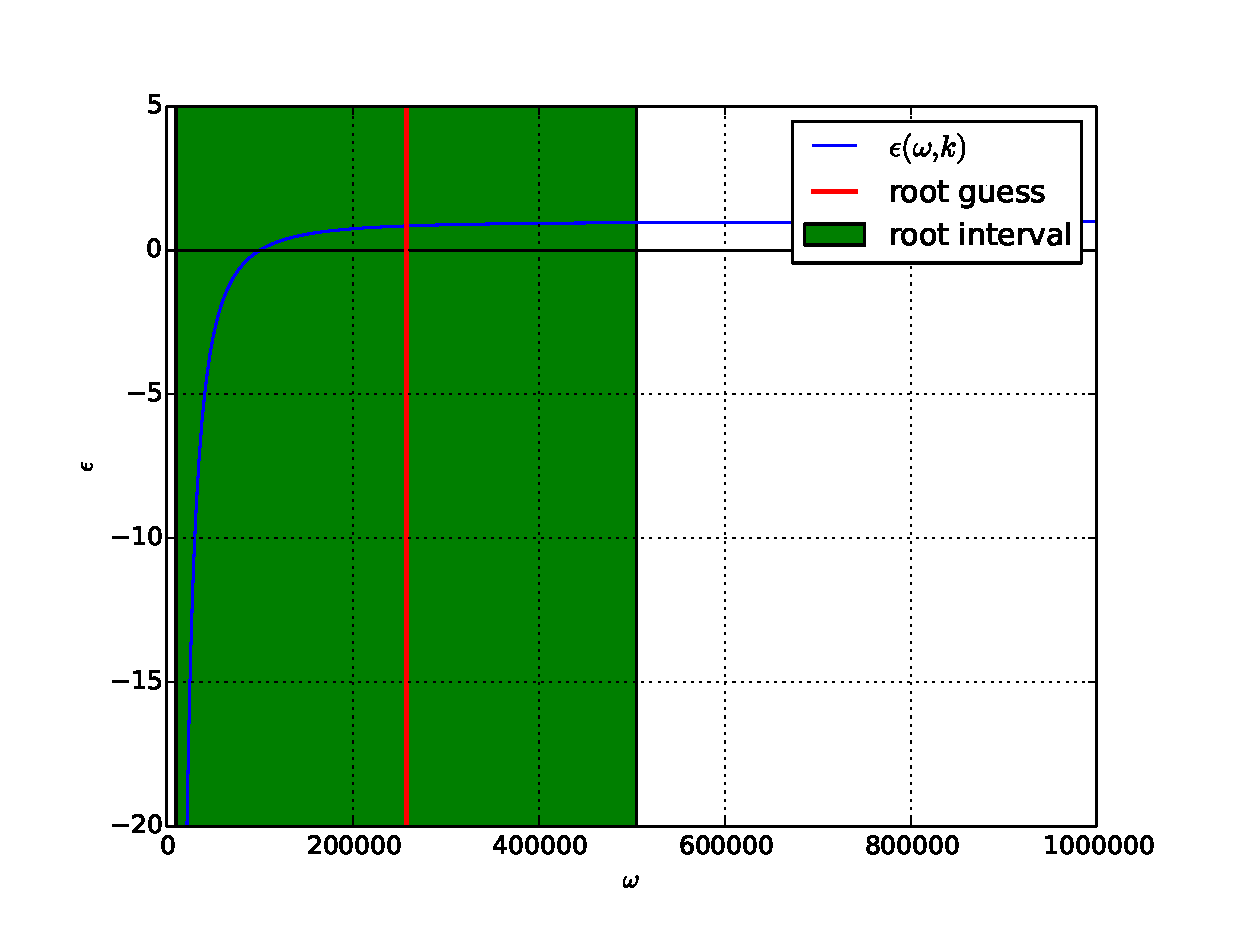
\includegraphics[width = 0.45\textwidth]{figures/bisection_100_0}
    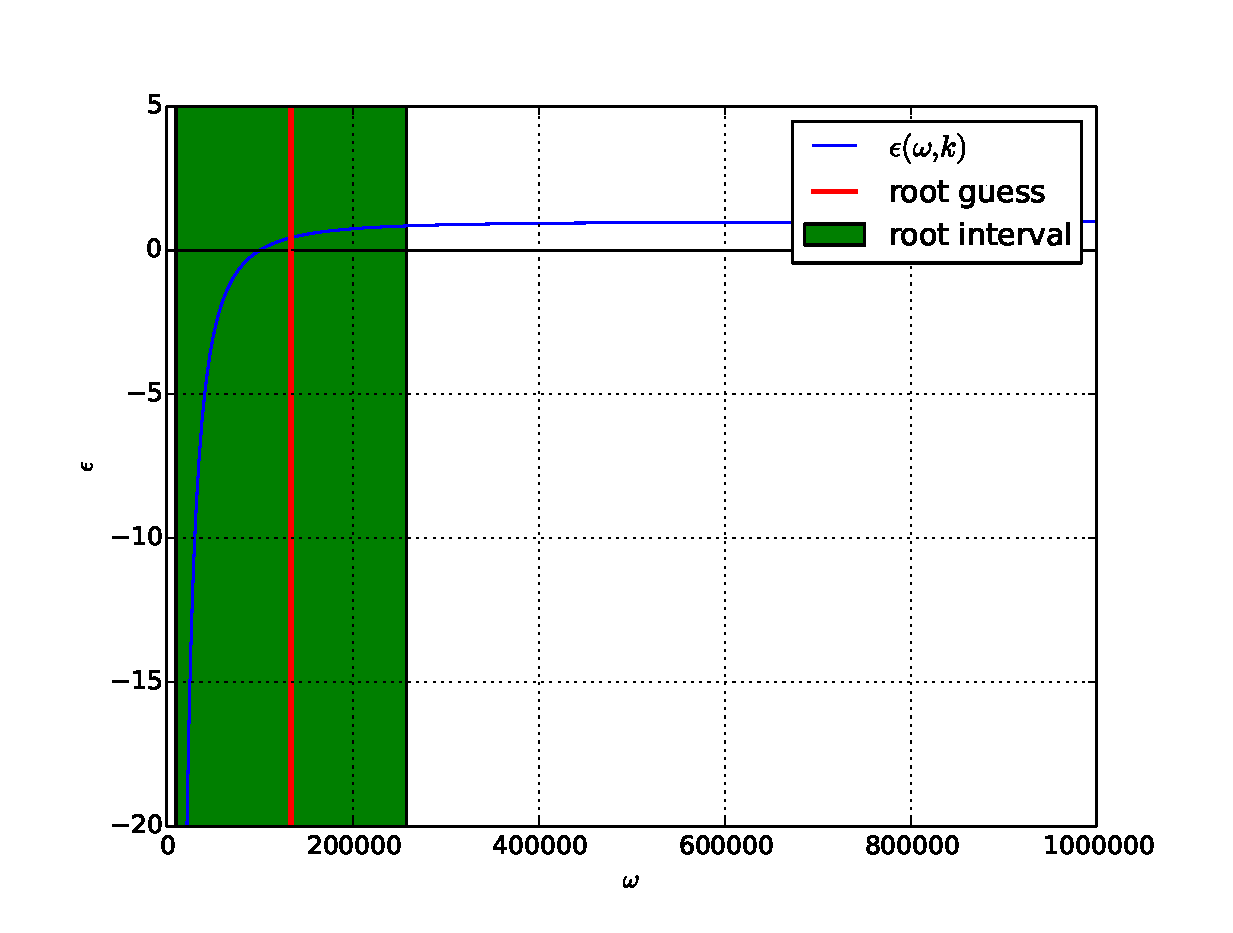
\includegraphics[width = 0.45\textwidth]{figures/bisection_100_1}
    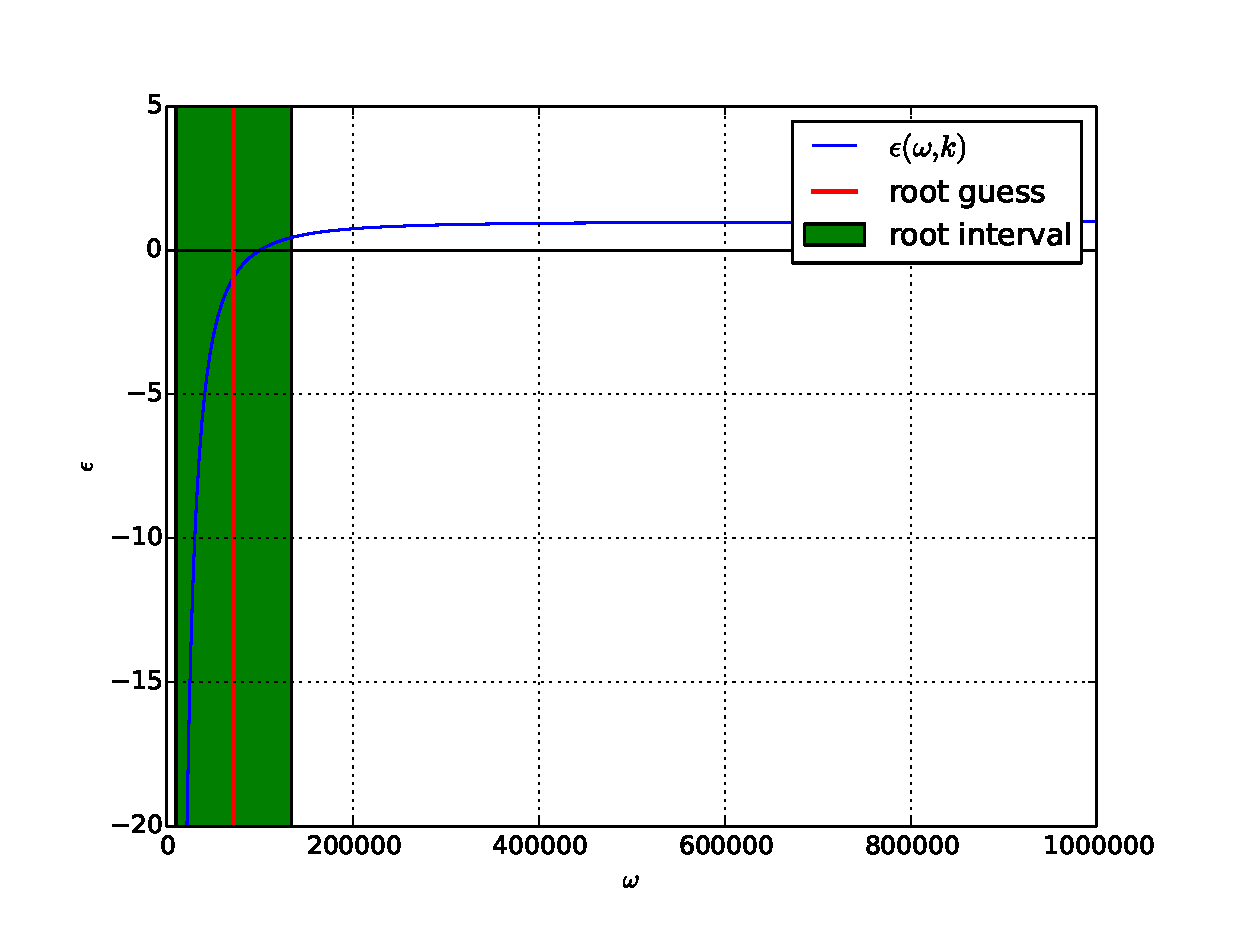
\includegraphics[width = 0.45\textwidth]{figures/bisection_100_2}
    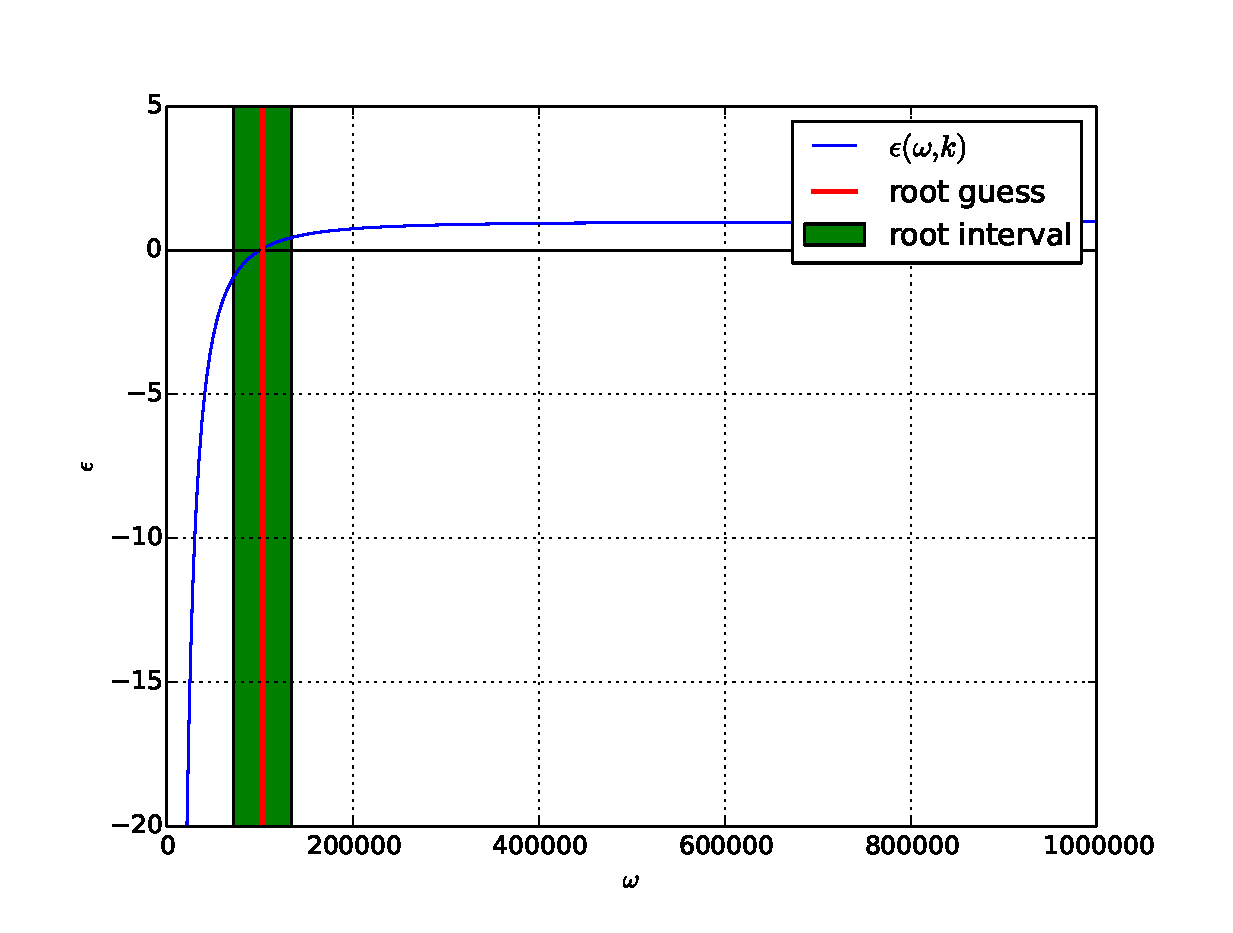
\includegraphics[width = 0.45\textwidth]{figures/bisection_100_3}
    \caption{Figures showing how the bisection method is searching for where the root is for a given function \(\epsilon\). It starts with a guess that the root is in \([0,5\times 10^5]\), then it divides that interval into the two intervals \([0,2.5\times 10^5)\) and \([2.5\times 10^5, 5\times 10^5]\), depicted in the uppermost left figure, and then it decides which interval the root lies on (colored green in the figure). Then it divides that interval in two again, (uppermost right figure) and repeats.}
    \label{fig:bisection}
  \end{figure}

\subsection{Results}
  To test the root finding algorithm we also used the dispersion relation, given in \cref{sec:elec_plasma}, and the dispersion diagram of it is depicted in \cref{fig:simple_diagram}. 

  \begin{figure}
  \centering
    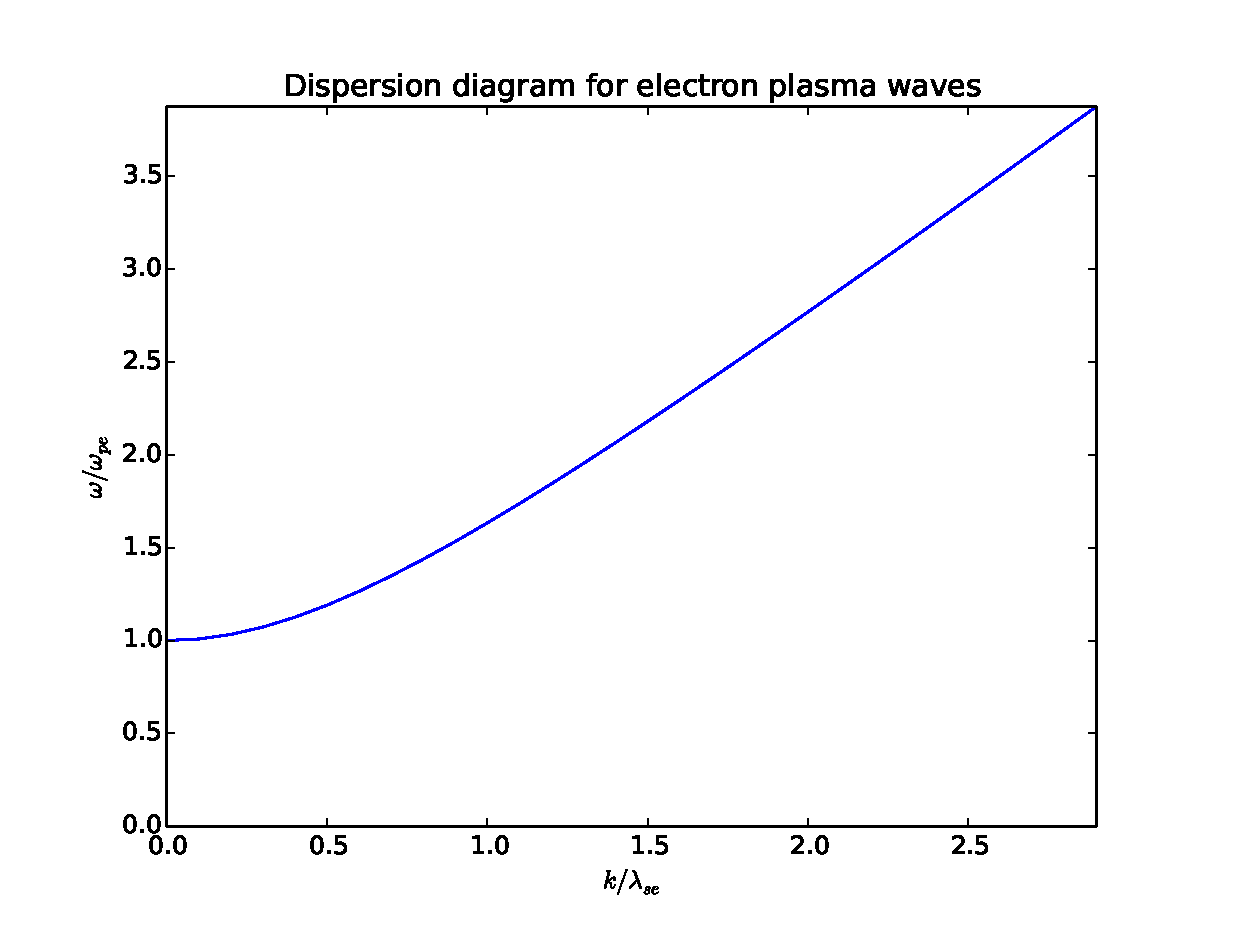
\includegraphics[width = 0.60 \textwidth]{figures/simple_dispersion}
    \caption{We see at large wavelengths the dispersion relation corresponds to a linear relation between the frequency and wave-vector.}
    \label{fig:simple_diagram}
  \end{figure}


  The dispersion relation for the ion acoustic waves, described in \cref{eq:dispersion_relation}, is shown in \cref{fig:ionAcousticDispers}. The second term, \(\frac{k^2c^2}{\omega^2}\), is dominating the equation, so the dispersion relation is almost linear for the wavenumber domain.
  \begin{figure}
  \centering
    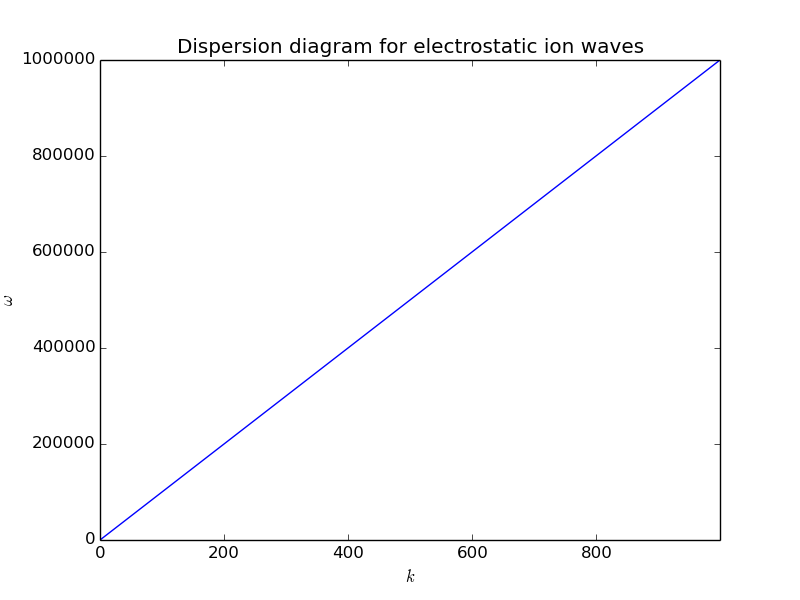
\includegraphics[width = 0.60 \textwidth]{figures/ionAcousticWaves}
    \caption{This figure shows the dispersion relation for the ion acoustic waves.}
    \label{fig:ionAcousticDispers}
  \end{figure}

\newpage
\appendix
\section{Electron plasma oscillations in unmagnetized plasma}
  \label{sec:elec_plasma}
    Here we will consider an electron fluid under local thermal equilibrium, LTE, experiencing small perturbations from an equilibrium state of an homogeneous electron density, \(n_0\), and pressure, \(p_0\), and vanishing flow, \(\va{u}_0 = 0\), and electric field, \(\va{E}_0 = 0 \).
    The fluid is governed by the following equations:

    \begin{subequations}
      \begin{equation}
        \pdv{n_e}{t} + \nabla \cdot (n_e \va{u}_e) = 0 
      \end{equation}
      \begin{equation}
        m_en_e\left( \pdv{}{t} + \va{u}_e \cdot \nabla \right)\va{u}_e = e n_e \nabla \phi - \nabla p_e
      \end{equation}
      \begin{equation}
        \left( \pdv{}{t} + \va{u}_e \cdot \nabla \right) p_e + \frac{5}{3} p_e\nabla \cdot \va{u}_e = 0
      \end{equation}
      \begin{equation}
        \epsilon_0 \nabla^2 \phi = e\left( n_e - n_0 \right)
      \end{equation}
    \end{subequations}

  Assuming a small perturbation to the equilibrium.
  \begin{equation*}
  \text{Perturbation} \rightarrow
    \begin{cases}
      n_e = n_0 + \tilde{n}_e\\
      p_e = p_0 + \tilde{p}_e\\
      \va{u}_e = \tilde{\va{u}}_e\\
      \phi = \tilde {\phi}
    \end{cases}
  \end{equation*}

  Linearizing the equations after inserting the perturbation we get

  \begin{subequations}
      \begin{equation}
        \pdv{\tilde{n}_e}{t} + \nabla \cdot (n_0 \tilde{\va{u}}_e) = 0 \label{eq:continuity}
      \end{equation}
      \begin{equation}
        m_e \pdv{\tilde{\va{u}}_e}{t}  = e  \nabla \tilde{ \phi} - \frac{\nabla \tilde{p}_e}{n_0}
      \end{equation}
      \begin{equation}
         \pdv{\tilde{p}}{t} +\frac{5}{3}p_0 \nabla \cdot \tilde{\va{u}}_e = 0 \label{eq:energy}
      \end{equation}
      \begin{equation}
        \epsilon_0 \nabla^2 \tilde{\phi} = e\tilde{n}_e
      \end{equation}
  \end{subequations}

  Combining the continuity and energy equations, \cref{eq:continuity} and \cref{eq:energy}, we get

  \begin{align}
    \pdv{}{t}\left( \frac{\tilde{p}_e}{p_0} + \frac{5}{3} \frac{\tilde{n_e}}{n_0} \right) &= 0
  \end{align}

  \noindent Assuming plane wave solutions and some algebra, we arrive at a compressional dispersal relation 

  \begin{align}
    \epsilon(\omega, k) = 1 + \frac{5}{3} \lambda_{se}^2k ^2 -  \frac{\omega^2}{\omega_{pe}^2} 
  \end{align}


\section{Comments to Exercise}
  
  \begin{itemize}
    \item Typo in dispersion relation, second term: \(\frac{k^2c_s^s}{\omega^2}\) should be \(\frac{k^2c_s^2}{\omega^2}\). (The \(c_s\) is raised to the power s instead of 2)
    \item Would it be an idea to start with a simple dispersion relation, implement the root finding algorithm on that, and then put in the complicated dispersion relation. An easy dispersion relation would be the one for electron oscillations in an unmagnetized plasma.
    \begin{align}
      \epsilon(\omega, k) &= 1 + \frac{5}{3}k^2 - \frac{\omega}{\omega_{pe}}
    \end{align}
    \item Is it necessary to look at the graph and guess an approximate interval? It's very fast to just do 50 iterations of the root finding algorithm which should give plenty of accuracy in the answer. I can see a point to confirm that it passes the x-axis.
    \item I can't get the third term of the dispersion relation to actually influence it, the ratio between them is typically of the \(10^15\) order. The relevant code follows:
      \begin{lstlisting}
      def epsilon(omega, k):
      cs  = 1000              #m/s    Speed of sound
      O_i = 300               #1/s    Ion gyrating frequency
      O_e = 8.E6              #1/s    Electron gyrating frequency
      theta = np.deg2rad(10)  #rad    angle between propagation and B
      tan2theta = np.tan(theta)**2


      return 1 - (k*k*cs*cs)/(omega*omega) + O_i*tan2theta/omega*(
              1/( omega*tan2theta/O_e  -  O_e/omega *(1 - omega*omega/O_e) ) -
              1/( omega*tan2theta/O_i  -  O_i/omega *(1 - omega*omega/O_i) )  )
      \end{lstlisting}



  \end{itemize}


\section{Code}
  \label{sec:code}
  \lstinputlisting{../source/dispersion.py}


\end{document}